% ---------------------------------------------------------------------------
% Interior del reparto por TDEST entre el puente VHDL y el MCDMA: cómo un
% único par de interfaces AXI-Stream da servicio a los catorce canales serie,
% con el puente etiquetando en recepción y el MCDMA demultiplexando por esa
% etiqueta hacia el buffer de la DDR que corresponde.
% Fuente del PDF que incluye la memoria (capítulo 3).
%
% Compilar:  pdflatex diagrama_mcdma_interior.tex
% ---------------------------------------------------------------------------
\documentclass[border=8pt]{standalone}
\usepackage[utf8]{inputenc}
\usepackage[T1]{fontenc}
\usepackage{lmodern}
\usepackage{tikz}
\usetikzlibrary{arrows.meta, calc}

\definecolor{cPropio}{HTML}{2A78D6}   % azul: lógica de diseño propio
\definecolor{cIP}{HTML}{EDA100}       % ámbar: IP de terceros
\definecolor{cExt}{HTML}{1BAF7A}      % aguamarina: software y hardware externo
\definecolor{cRef}{HTML}{8A8A85}      % gris: líneas, bandas y contornos

\begin{document}
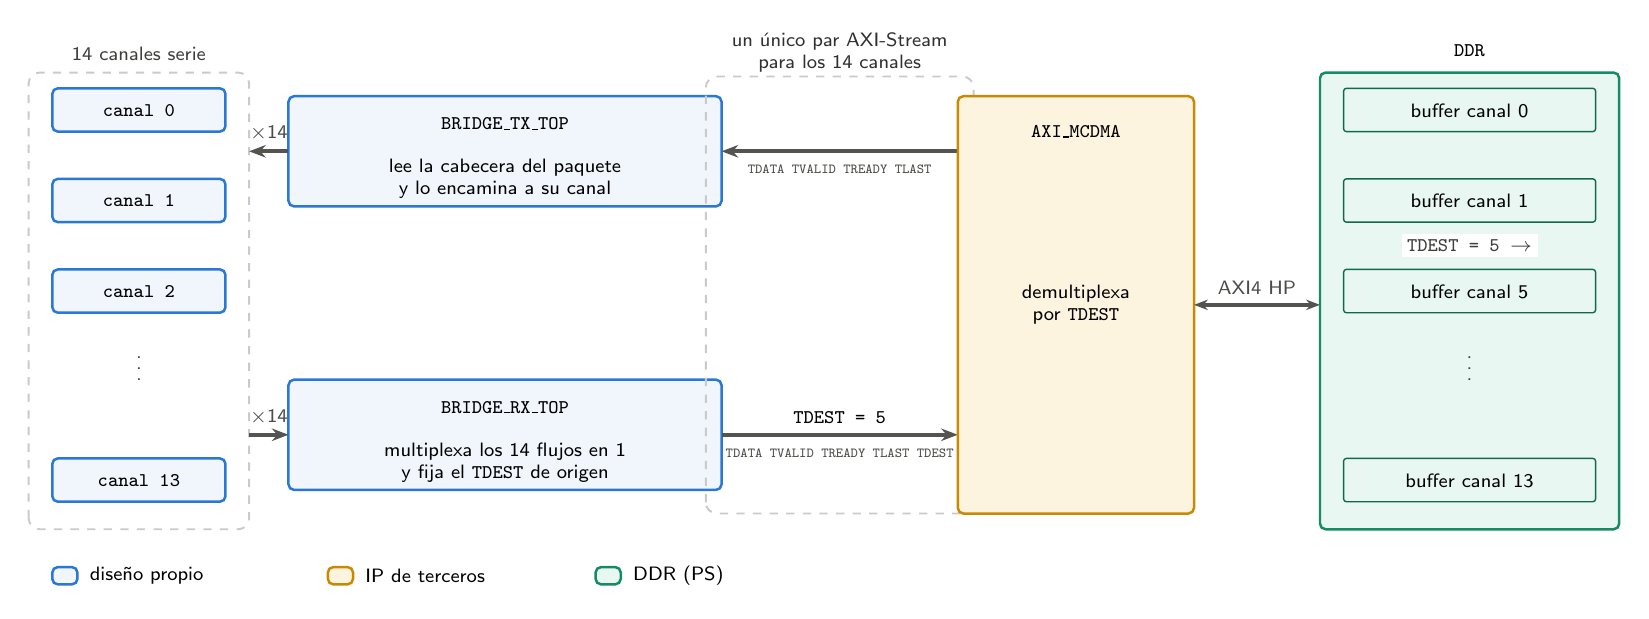
\begin{tikzpicture}[
    x=1cm, y=1cm, font=\sffamily\small,
    blk/.style={draw=cPropio, line width=0.9pt, rounded corners=2pt,
                fill=cPropio!7},
    ip/.style={draw=cIP!85!black, line width=0.9pt, rounded corners=2pt,
               fill=cIP!12},
    ext/.style={draw=cExt!80!black, line width=0.9pt, rounded corners=2pt,
                fill=cExt!10},
    band/.style={draw=cRef!45, dashed, line width=0.7pt, rounded corners=4pt},
    sig/.style={-{Stealth[length=4.5pt]}, line width=0.7pt, cRef!85!black},
    stream/.style={-{Stealth[length=6pt]}, line width=1.5pt, cRef!60!black},
    irq/.style={-{Stealth[length=4.5pt]}, line width=0.7pt, cIP!70!black},
    lbl/.style={font=\sffamily\scriptsize, inner sep=2pt},
    tlbl/.style={font=\ttfamily\scriptsize, inner sep=2pt},
    name/.style={font=\ttfamily\scriptsize, align=center},
]

% ===================== Catorce canales serie =====================
\draw[band] (0.2,3.8) rectangle (3.0,9.6);
\node[lbl, anchor=south, text=cRef!45!black] at (1.6,9.68) {14 canales serie};

\draw[blk] (0.5,8.85) rectangle (2.7,9.40);
\node[name] at (1.6,9.12) {canal 0};
\draw[blk] (0.5,7.70) rectangle (2.7,8.25);
\node[name] at (1.6,7.97) {canal 1};
\draw[blk] (0.5,6.55) rectangle (2.7,7.10);
\node[name] at (1.6,6.82) {canal 2};
\node[lbl, text=cRef!45!black] at (1.6,5.95) {$\vdots$};
\draw[blk] (0.5,4.15) rectangle (2.7,4.70);
\node[name] at (1.6,4.42) {canal 13};

% ===================== Puente VHDL: transmisión (arriba) =====================
\draw[blk] (3.5,7.90) rectangle (9.00,9.30);
\node[name] at (6.25,8.95) {BRIDGE\_TX\_TOP};
\node[lbl, align=center] at (6.25,8.25) {lee la cabecera del paquete\\y lo encamina a su canal};

% ===================== Puente VHDL: recepción (abajo) =====================
\draw[blk] (3.5,4.30) rectangle (9.00,5.70);
\node[name] at (6.25,5.35) {BRIDGE\_RX\_TOP};
\node[lbl, align=center] at (6.25,4.65) {multiplexa los 14 flujos en 1\\y fija el \texttt{TDEST} de origen};

% ===================== Conexión canales <-> puente =====================
\draw[stream] (3.5,8.60) -- (3.0,8.60);
\draw[stream] (3.0,5.00) -- (3.5,5.00);
\node[lbl, anchor=south, text=cRef!55!black] at (3.25,8.65) {$\times$14};
\node[lbl, anchor=south, text=cRef!55!black] at (3.25,5.05) {$\times$14};

% ===================== Único par AXI-Stream puente <-> MCDMA =====================
\draw[band] (8.80,4.00) rectangle (12.20,9.55);
\node[lbl, align=center, text=cRef!35!black] at (10.50,9.85)
      {un único par AXI-Stream\\para los 14 canales};

\draw[stream] (12.00,8.60) -- (9.00,8.60);
\node[font=\ttfamily\tiny, text=cRef!55!black, anchor=north, inner sep=2pt]
      at (10.50,8.50) {TDATA TVALID TREADY TLAST};

\draw[stream] (9.00,5.00) -- (12.00,5.00);
\node[font=\ttfamily\tiny, text=cRef!55!black, anchor=north, inner sep=2pt]
      at (10.50,4.90) {TDATA TVALID TREADY TLAST TDEST};
\node[tlbl, anchor=south, fill=white, inner sep=2pt] at (10.50,5.06)
      {\texttt{TDEST = 5}};

% ===================== MCDMA =====================
\draw[ip] (12.00,4.00) rectangle (15.00,9.30);
\node[name] at (13.50,8.85) {AXI\_MCDMA};
\node[lbl, align=center] at (13.50,6.65) {demultiplexa\\por \texttt{TDEST}};

% ===================== MCDMA <-> DDR =====================
\draw[{Stealth[length=5pt]}-{Stealth[length=5pt]}, line width=1.5pt, cRef!60!black]
      (15.00,6.65) -- (16.60,6.65);
\node[lbl, anchor=south, text=cRef!55!black] at (15.80,6.70) {AXI4 HP};

% ===================== DDR con un buffer por canal =====================
\draw[ext] (16.60,3.80) rectangle (20.40,9.60);
\node[name, anchor=south] at (18.50,9.68) {DDR};

\draw[draw=cExt!60!black, line width=0.5pt, rounded corners=1pt]
      (16.90,8.85) rectangle (20.10,9.40);
\node[lbl] at (18.50,9.12) {buffer canal 0};
\draw[draw=cExt!60!black, line width=0.5pt, rounded corners=1pt]
      (16.90,7.70) rectangle (20.10,8.25);
\node[lbl] at (18.50,7.97) {buffer canal 1};
\node[tlbl, fill=white, inner sep=2pt, text=cRef!45!black] at (18.50,7.40)
      {\texttt{TDEST = 5} $\rightarrow$};
\draw[draw=cExt!60!black, line width=0.5pt, rounded corners=1pt]
      (16.90,6.55) rectangle (20.10,7.10);
\node[lbl] at (18.50,6.82) {buffer canal 5};
\node[lbl, text=cRef!45!black] at (18.50,5.95) {$\vdots$};
\draw[draw=cExt!60!black, line width=0.5pt, rounded corners=1pt]
      (16.90,4.15) rectangle (20.10,4.70);
\node[lbl] at (18.50,4.42) {buffer canal 13};

% ===================== Leyenda =====================
\draw[blk] (0.5,3.10) rectangle (0.82,3.32);
\node[lbl, anchor=west] at (0.90,3.21) {diseño propio};
\draw[ip] (4.0,3.10) rectangle (4.32,3.32);
\node[lbl, anchor=west] at (4.40,3.21) {IP de terceros};
\draw[ext] (7.4,3.10) rectangle (7.72,3.32);
\node[lbl, anchor=west] at (7.80,3.21) {DDR (PS)};

\end{tikzpicture}
\end{document}
